\documentclass[12pt,oneside]{article}
\usepackage{geometry}                                % See geometry.pdf to learn the layout options. There are lots.
\usepackage{listings}				% Permite utilizar lenguajes de programacion dentro de latex
\geometry{a4paper}                                           % ... or a4paper or a5paper or ... 
%\geometry{landscape}                                % Activate for for rotated page geometry
%\usepackage[parfill]{parskip}                    % Activate to begin paragraphs with an empty line rather than an indent
\usepackage{graphicx}                                % Use pdf, png, jpg, or epsß with pdflatex; use eps in DVI mode
                                                                % TeX will automatically convert eps --> pdf in pdflatex                
\usepackage{amssymb}

\usepackage[spanish]{babel}                        % Permite que partes automáticas del documento aparezcan en castellano.
\usepackage[utf8]{inputenc}                        % Permite escribir tildes y otros caracteres directamente en el .tex
\usepackage[T1]{fontenc}                                % Asegura que el documento resultante use caracteres de una fuente apropiada.

\usepackage{hyperref}                                % Permite poner urls y links dentro del documento
\usepackage{listings}

\title{Ejercicios de Programación - Sebesta}
\author{Lenguajes de Programación - ESPOL}

%\date{}                                                        % Activate to display a given date or no date

\begin{document}
\maketitle

	\section{Introducción}
	Las respuestas propuestas en este repositorio son producto del trabajo de los estudiantes de la materia ``Lenguajes de Programación'' de la ESPOL, correspondientes a las preguntas del libro de Robert Sebesta, Concepts of Programming Languages.

	\section{Preguntas y Respuestas}

		\subsection{Capítulo 5: Nombres, Enlaces y Alcances}
			\begin{itemize}
				\item {\bf Pregunta 4}	
				OJOOOOOOOOOO faltaaaaaaaaaaaaaaaaaaa

				\item {\bf Pregunta 5: Write a C function that includes the following sequence of statements: x = 21;int x;x = 42; Run the program and explain the results. Rewrite the same code in C++ and Java and compare the results.}
					\begin{itemize}
						\item {Función en C}
							\begin{center}
							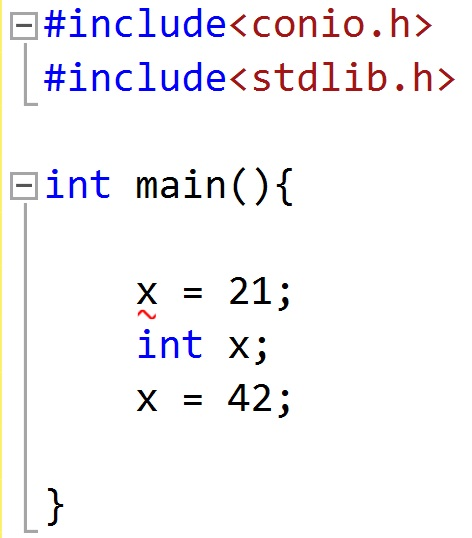
\includegraphics[scale=0.3]{Imagenes/1.jpg}\\
							NO COMPILA: error C2065: 'x' : identificador no declarado
							\end{center}
							ARGUMENTO: En el lenguaje C es necesario crear la variable o instanciarla de las siguientes formas antes de poder usarla o asignarle un valor: 
							\begin{itemize}
								\item{(tipo) (nombreVariable);}
									\\Ejemplo: int x;
								\item{(tipo) (nombreVariable)=(valor Inicial);}		
									\\Ejemplo: int x=10;							
							\end{itemize}

						\item {Función en C++}
							\\Sucede lo mismo que en C, el compilador de visual presenta los mismos errores, como si las tres lineas estuvieran mal escritas, aunque realmente es la primera.

						\item {Función en Java}
							\begin{center}
							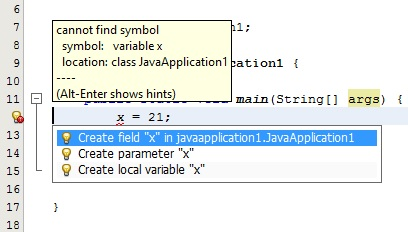
\includegraphics[scale=0.9]{Imagenes/2.jpg}\\
							NO COMPILA: error: cannot find symbol
							\end{center}		
							ARGUMENTO: En el lenguaje Java, el intérprete antes de compliar sugiere al programador crear la variable X como una variable de clase, y una vez compilado muestrar el error de que no puede encontrar el simbolo que se esta 									intentado usar, en este caso X.									
					\end{itemize}

				\item {\bf Pregunta 6: Write test programs in C++, Java, and C\# to determine the scope of a variable declared in a for statement. Specifically, the code must determine whether such a variable is visible after the body of the for statement.}
					\begin{itemize}
						\item {Función en C++}
							\begin{center}
								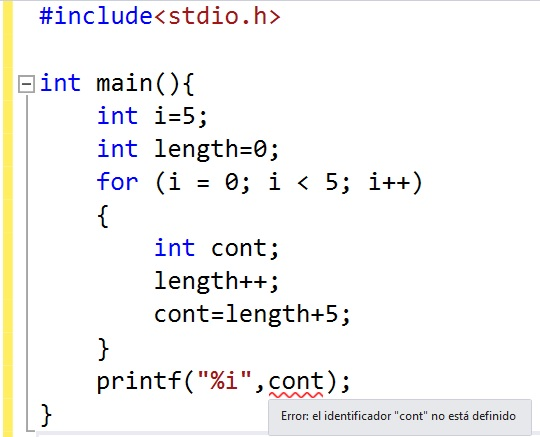
\includegraphics[scale=0.6]{Imagenes/3.jpg}\\
								NO COMPILA: No es visible despues de la sentencia for.
							\end{center}
						\item {Función en C\#}
							\begin{center}
								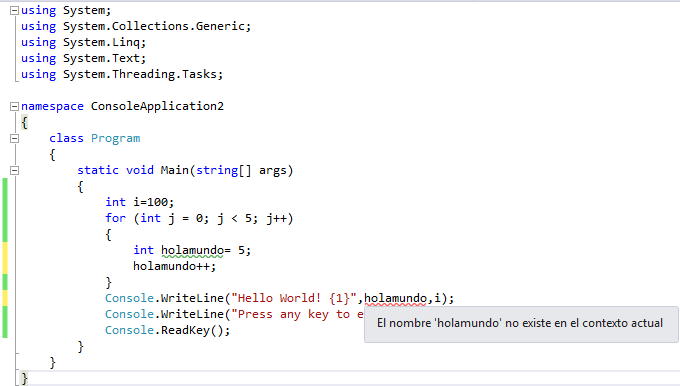
\includegraphics[scale=0.8]{Imagenes/4.jpg}\\
								NO COMPILA: No es visible despues de la sentencia for.
							\end{center}
							Es de notar que los avisos que muestra el intérprete son diferentes en los dos casos anteriores, en C++ nos dice que no existe definición de la variable que se quiere usar y por tanto no hay ningún valor que mostrar. En la 									siguiente, en C\# en cambio nos informa que no estamos en el mismo contexto y que por tanto la variable no es visible ni alcanzable.
					\end{itemize}
				\item {\bf Pregunta 7}	
					OJOOOOOOOOOO faltaaaaaaaaaaaaaa
		\end{itemize}


		\subsection{Capítulo 6: Tipos de Datos}
			\begin{itemize}
				\item {\bf Pregunta 1}
					OJOOOOOOOOOO faltaaaaaaaaaaaaaaaaaaaaa
				\item {\bf Pregunta 2}
					OJOOOOOOOOOO faltaaaaaaaaaaaaaaaaaaa
				\item {\bf Pregunta 7}
					OJOOOOOOOOOO faltaaaaaaaaaaaaaa
				\end{itemize}

		\subsection{Capítulo 7: Expresiones e Instrucciones de asignación}	
			\begin{itemize}
				\item {\bf Pregunta 1}
					OJOOOOOOOOOO faltaaaaaaaaaaaaaaaaa
				\item {\bf Pregunta 2}
					OJOOOOOOOOOO faltaaaaaaaaaaaaaaaaaa
				\item {\bf Pregunta 3}
					OJOOOOOOOOOO faltaaaaaaaaaaaaaaaa
				\item {\bf Pregunta 4}
					OJOOOOOOOOOO faltaaaaaaaaaaaaaaaaaa
				\item {\bf Pregunta 5}
					OJOOOOOOOOOO faltaaaaaaaaaaaaaaa
				\item {\bf Pregunta 6}
					OJOOOOOOOOOO faltaaaaaaaaaaaaaaaaa
				\item {\bf Pregunta 9}
					OJOOOOOOOOOO faltaaaaaaaaaaaaaaaaa
				\end{itemize}

		\subsection{Capítulo 8: Estructuras de Control}	
			\begin{itemize}
				\item {\bf Pregunta 3}		
					OJOOOOOOOOOO faltaaaaaaaaaaaaaaaa
				\item {\bf Pregunta 4}
					OJOOOOOOOOOO faltaaaaaaaaaaaaaaaaaaaaaa
				\item {\bf Pregunta 5}
					OJOOOOOOOOOO faltaaaaaaaaaaaaaaaaaaaaaaa
			\end{itemize}

		\subsection{Capítulo 9: SubProgramas}      
			\begin{itemize}
				\item {\bf Pregunta 1}
					OJOOOOOOOOOO faltaaaaaaaaaaaaaaaaaaaaaa
				\item {\bf Pregunta 5}
					OJOOOOOOOOOO faltaaaaaaaaaaaaaaaaaaaaaaa
				\end{itemize}


% Continuar con los siguientes capítulos y ejercicios:
% Ch6: 1, 2, 7
% Ch7: 1 - 6, 9
% Ch8: 3, 4, 5
% Ch9: 1, 5
% Recuerden que todos corresponden a las secciones de "Programming Exercises".

\end{document}
